Thinking...
The user wants translation of Japanese text to English, but TeX code should be left as is. The Japanese text includes the figure environment with caption etc. Need to translate the Japanese text outside the TeX code? The whole snippet is TeX code, but the caption contains Japanese. So we translate caption and maybe other parts? The instruction: "以下のの日本語文を英訳してください。ただしTeXのコードが挿入されているのでその部分はそのまま出力してください。" Means: Translate the Japanese sentences into English, but the TeX code parts should be output as is.

Thus we need to keep the entire TeX environment unchanged except we replace Japanese text with English equivalents. Which parts are Japanese? The caption text: "被引用減衰が確認された高被引用論文の階層クラスタリングとPCAプロット". Also maybe "fig:gr8"? That's label; keep unchanged. The rest is TeX commands.

So output should be same block but with caption replaced with English translation. Translate: "Hierarchical clustering and PCA plot of highly cited papers where citation decay has been confirmed." Something like that.

Thus final answer:

\begin{figure*}[h]
\begin{center}
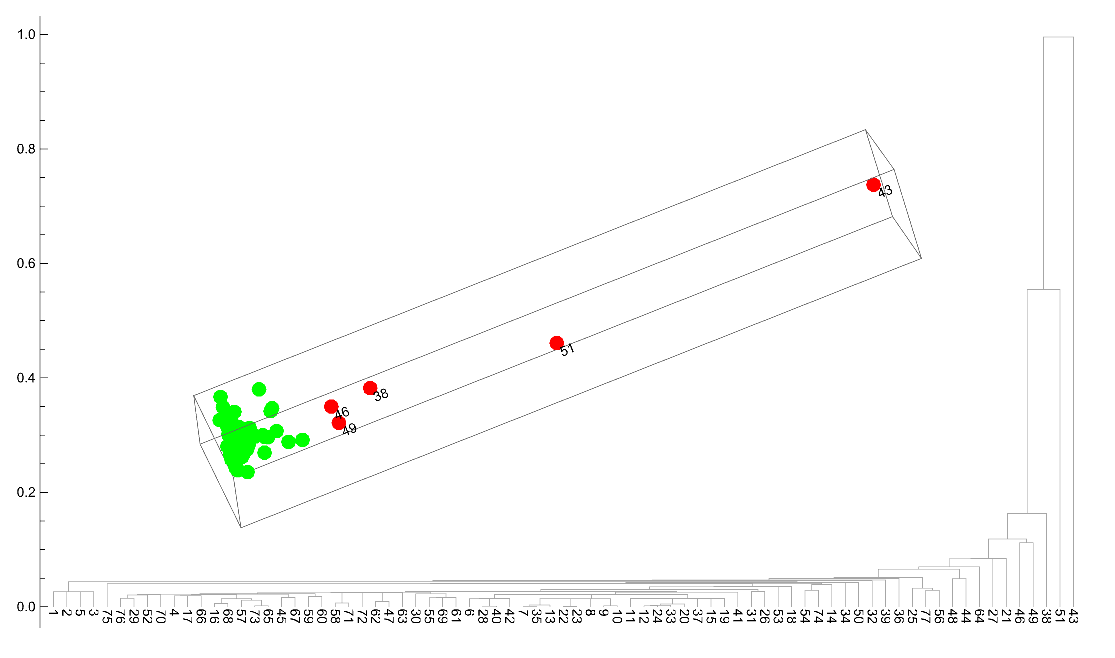
\includegraphics[width=160mm]{gr8.eps}
\caption{Hierarchical clustering and PCA plot of highly cited papers in which citation decay was confirmed}
\label{fig:gr8}
\end{center}
\end{figure*}

Provide that.
...done thinking.

\begin{figure*}[h] 
\begin{center} 
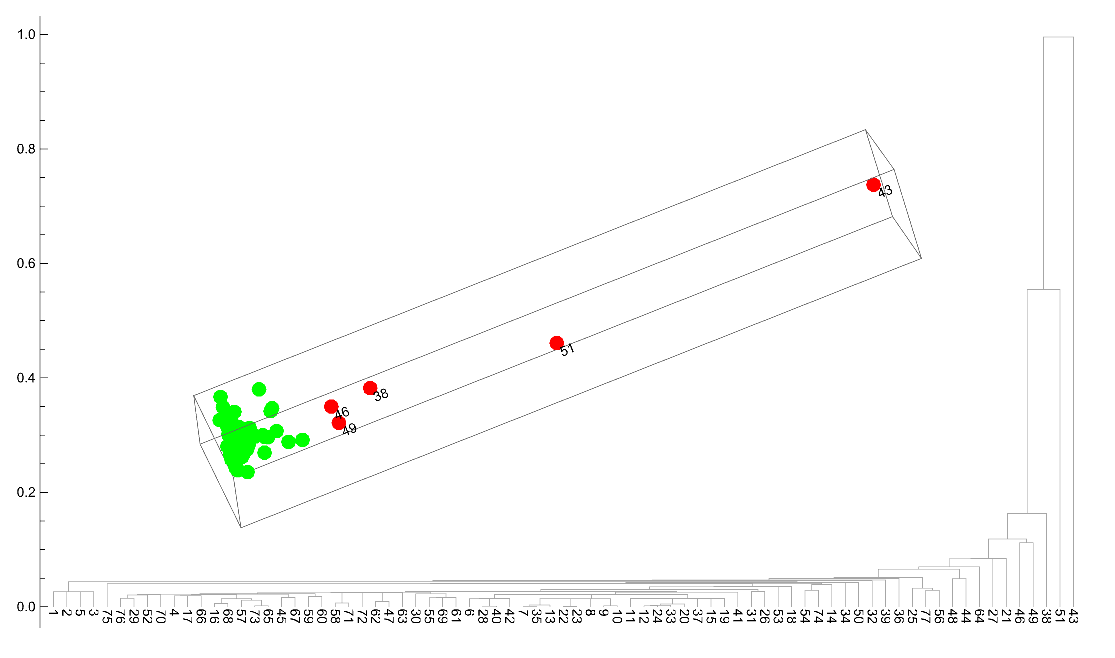
\includegraphics[width=160mm]{gr8.eps} 
\caption{Hierarchical clustering and PCA plot of highly cited papers in which citation decay was confirmed} 
\label{fig:gr8} 
\end{center} 
\end{figure*}

